% Evans 6.3: English printed p.307 / PDF p.324; Chinese printed p.218 / PDF p.236.
\Needspace{65mm}
\section{Regularity}
\label{sec:6-3}
\subsection{Interior energy localization}
Throughout the $H^2$ argument, $A\in C^1(U)$ is uniformly elliptic,
$b,c\in L^\infty_{\mathrm{loc}}(U)$, $f\in L^2_{\mathrm{loc}}(U)$, and
$u\in H^1(U)$ solves $Lu=f$ against compactly supported tests.
All coefficient bounds below are on a fixed relatively compact region.

\begin{lemma}[Caccioppoli estimate]\label{lem:6-caccioppoli}
For a smooth cutoff $0\leq\eta\leq1$ with compact support in $U$,
\[
 \int_U\eta^2|Du|^2
 \leq C\int_{\operatorname{supp}\eta}
 \bigl(|f|^2+(1+|D\eta|^2)|u|^2\bigr).
\]
\end{lemma}
\begin{expandedproof}
The admissible test $\eta^2u$ gives
\[
 \int\eta^2 A Du\cdot Du
 =\int f\eta^2u-2\int\eta u\, A Du\cdot D\eta
       -\int b\cdot Du\,\eta^2u-\int c\eta^2u^2.
\]
The second and third terms are bounded, for any $\varepsilon>0$, by
\[
 \varepsilon\int\eta^2|Du|^2+
 C_\varepsilon\int(|D\eta|^2+\eta^2)u^2.
\]
Use $|fu|\leq(f^2+u^2)/2$, bound the potential term, and choose
the two $\varepsilon$'s so their sum is less than $\theta/2$.
Move these gradient terms to the left.
\end{expandedproof}
\Needspace{45mm}
\PDEAnnotation{截断函数的代价}{局部估计中出现 $D\eta$，所以常数依赖内外区域的距离。把内区推向边界会使常数变大，不能把内部估计直接当成全局边界估计。}

\Needspace{35mm}
\subsection{Interior $H^2$ regularity (Evans \S6.3.1, Theorem 1)}
\begin{theorem}\label{thm:6-interior-h2}
For $V\Subset U$, a weak solution as above belongs to $H^2(V)$ and
\[
 \|u\|_{H^2(V)}
 \leq C\bigl(\|f\|_{L^2(W)}+\|u\|_{L^2(W)}\bigr),
 \qquad V\Subset W\Subset U.
\]
Here $C$ depends on the nested regions, ellipticity and the local
$C^1$ norm of $A$ and $L^\infty$ norms of $b,c$.
Local Lipschitz bounds on $A$ suffice for this proof.
\end{theorem}
\begin{expandedproof}
\paragraph{1. Choose a legal discrete substitute for a second derivative.}
Fix a coordinate direction $e_k$ and set
$\delta_h z(x)=[z(x+he_k)-z(x)]/h$ for either sign of $h$.
Choose $\eta=1$ on $V$, compactly supported in an intermediate region,
and $|h|$ small enough that all translated supports remain in $W$.
For fixed $h$,
\[
 q=\eta^2\delta_h u\in H^1_0(W),\qquad
 v=-\delta_{-h}q\in H^1_0(W).
\]
The difference quotient is in $H^1$ for fixed $h$ even though its
$H^1$ norm has not yet been bounded uniformly. Thus $v$ is a valid test.

\Needspace{45mm}
\PDEAnnotation{不能先假定二阶导数}{直接测试 $-\partial_{kk}u$ 会预先要求尚未证明的正则性。固定步长的差商仍在 $H^1$ 中，先合法计算，再用一致估计令步长趋零。}

\PDEBodyDiagram{6.3}{Localize before taking differences.}
{The cutoff equals one on $V$ and is supported strictly inside $W$. A fixed geometric gap permits all sufficiently small positive and negative steps. The support condition is settled before the estimate; the estimate's constant must then stay independent of $h$ as $h\to0$.}
{ch06-cutoff-translates}

\paragraph{2. Discrete integration by parts.}
A change of variables, with no support crossing the boundary, gives
\[
 \int g\,\delta_{-h}q=-\int(\delta_h g)q.
\]
Absorb lower-order terms into
$\widetilde f=f-b\cdot Du-cu\in L^2(W)$. The weak equation becomes
\[
 \int\delta_h(a^{ij}u_i)\,\partial_j(\eta^2\delta_hu)
       =-\int\widetilde f\,\delta_{-h}(\eta^2\delta_hu).
\]
The exact product rule is
\[
 \delta_h(a^{ij}u_i)
 =a^{ij}(x+he_k)\delta_hu_i+(\delta_h a^{ij})u_i .
\]
The coefficient in the first term is translated and remains elliptic.

\paragraph{3. Estimate each error before absorbing it.}
Put $X=\|\eta\,\delta_h Du\|_2$ and
$Y=\|Du\|_{L^2(W)}+\|u\|_{L^2(W)}$.
The main term is at least $\theta X^2$.
Since $\|\delta_hu\|_2\leq\|\partial_k u\|_{L^2(W)}$ on the relevant
supports and $|\delta_h A|\leq\|DA\|_\infty$, the other terms on the
left are bounded by
\[
 CXY+CY^2\leq\varepsilon X^2+C_\varepsilon Y^2.
\]
For example the cutoff term is bounded by
$C\|\eta\delta_hDu\|_2\|D\eta\,\delta_hu\|_2$; the coefficient
commutator is bounded by
$C\|Du\|_2(X+\|\delta_hu\|_2)$.

For the right side, the difference quotient inequality applied to $q$
gives
\[
 \|\delta_{-h}q\|_2\leq\|\partial_kq\|_2
 \leq C(X+Y).
\]
Therefore it is at most
$\varepsilon X^2+C_\varepsilon(\|\widetilde f\|_2^2+Y^2)$.
Since $\|\widetilde f\|_2\leq C(\|f\|_2+Y)$, absorption yields
\begin{equation}\label{eq:6-dq-bound}
 \|\delta_h Du\|_{L^2(V)}^2
 \leq C\bigl(\|f\|_{L^2(W)}^2+\|u\|_{H^1(W)}^2\bigr),
\end{equation}
with $C$ independent of $h$.

\Needspace{45mm}
\PDEAnnotation{一致估计才能识别弱导数}{差商判别准则作用于每个一阶导数 $u_i$：各方向的 $\delta_hu_i$ 一致有界，就得到 $u_{ik}\in L^2$。只证明每个固定步长有限并没有用。}
\paragraph{4. Pass to weak derivatives and remove the first-order norm.}
The difference quotient criterion of Chapter~5 applied to each $u_i$
gives $u_{ik}\in L^2(V)$. Repeating in every direction proves $H^2$.
Apply \eqref{eq:6-dq-bound} on slightly larger nested regions and use
Lemma~\ref{lem:6-caccioppoli} there to bound $\|Du\|_2$ by $f$ and $u$.
This gives the stated estimate with only the $L^2$ norm of $u$.
\end{expandedproof}

\Needspace{35mm}
\subsection{Higher interior regularity (Evans \S6.3.1, Theorems 2--3)}
\begin{theorem}\label{thm:6-higher-interior}
Let $m\geq0$ be an integer, $A,b,c\in C^{m+1}(U)$, and
$f\in H^m_{\mathrm{loc}}(U)$. Then
$u\in H^{m+2}_{\mathrm{loc}}(U)$, with
\[
 \|u\|_{H^{m+2}(V)}
 \leq C\bigl(\|f\|_{H^m(W)}+\|u\|_{L^2(W)}\bigr),
 \quad V\Subset W\Subset U.
\]
Smooth coefficients and smooth $f$ give $u\in C^\infty(U)$.
\end{theorem}
\begin{expandedproof}
The case $m=0$ is proved. Suppose $u\in H^{m+2}$ on intermediate regions
and $f\in H^{m+1}$. For $|\alpha|=m+1$, differentiate the equation
in distributions. With $z=D^\alpha u\in H^1$,
\begin{align*}
 Lz={}&D^\alpha f+
 \sum_{0<\beta\leq\alpha}\binom{\alpha}{\beta}
 \partial_j\bigl((D^\beta a^{ij})
                \partial_iD^{\alpha-\beta}u\bigr)\\
 &-\sum_{0<\beta\leq\alpha}\binom{\alpha}{\beta}
 \bigl((D^\beta b^i)\partial_iD^{\alpha-\beta}u
       +(D^\beta c)D^{\alpha-\beta}u\bigr).
\end{align*}
Expand the divergence in the first line. Its highest derivative of $u$
has order $|\alpha|-|\beta|+2\leq m+2$, already known in $L^2$;
coefficient derivatives have order at most $m+2$.
Thus the entire right side lies in $L^2$. Interior $H^2$ regularity
for $z$ gives derivatives of $u$ through order $m+3$.
A finite chain of nested regions gives the norm bound inductively.
For any fixed $k$, choose a Sobolev order $s>k+n/2$ and use the
embedding $H^s_{\mathrm{loc}}\hookrightarrow C^k_{\mathrm{loc}}$.
Since $k$ is arbitrary, smoothness follows.
\end{expandedproof}
\Needspace{45mm}
\PDEAnnotation{提升正则性不是循环论证}{先由已知阶数判断交换子右端属于 $L^2$，再把二阶正则性定理用于导函数。光滑系数得到光滑解，并不自动得到解析解。}

% Supplement to Evans 6.3.2: expanded boundary localization and derivative recovery.
\Needspace{35mm}
\subsection{Boundary $H^2$ regularity (Evans \S6.3.2, Theorem 4)}
\begin{theorem}\label{thm:6-boundary-h2}
Suppose $\partial U$ is $C^2$, $A\in C^1(\overline U)$,
$b,c\in L^\infty(U)$ and $f\in L^2(U)$. A weak Dirichlet solution
$u\in H^1_0(U)$ belongs to $H^2(U)$ and satisfies
\[
 \|u\|_{H^2(U)}\leq C(\|f\|_2+\|u\|_2).
\]
If the Dirichlet operator is invertible, the last term can be removed.
\end{theorem}
\begin{expandedproof}

\Needspace{45mm}
\PDEAnnotation{正则性估计不等于可解性}{估计以解已经存在为前提。右边保留 $ \|u\|_2 $ 是为容纳有限维齐次核；只有先证明算子可逆，才能用右端独自控制整个解。}
\paragraph{1. A flat boundary permits tangential differences.}
Work first in a half-ball $B^+_r=\{x\in B_r:x_n>0\}$, where the trace of
$u$ is zero on $x_n=0$. Choose a cutoff vanishing near the curved boundary.
For $k<n$, tangential translation preserves the half-space and the zero
trace, so the test
$-\delta_{-h}(\eta^2\delta_hu)$ remains admissible.
The preceding calculation bounds every $u_{ik}$ with $k<n$ in $L^2$
on a smaller half-ball. This includes the mixed normal--tangential
derivatives, since distributional derivatives commute.

\Needspace{45mm}
\PDEAnnotation{法向差商为何失效}{沿边界平移不会越出半空间，也保留零迹；法向平移会穿过边界，测试函数不再合法。因此先求所有带切向指标的导数，最后用方程解出纯法向导数。}
\paragraph{2. Ellipticity recovers the missing derivative.}
Expand the divergence equation in distributions:
\begin{equation}\label{eq:6-normal-recovery}
 a^{nn}u_{nn}
 =-\sum_{(i,j)\ne(n,n)}a^{ij}u_{ij}
   +(b^i-\partial_j a^{ij})u_i+cu-f.
\end{equation}
Every term on the right is in $L^2$ by Step 1.
Because $a^{nn}\geq\theta$, division bounds $u_{nn}$.
One rigorous way to avoid assuming $H^2$ up to the boundary at this
step is to use the already proved interior $H^2$ theorem: the identity
holds almost everywhere away from $x_n=0$, and its right side has
a uniform $L^2$ bound on the whole smaller half-ball.
The resulting $L^2$ function is the distributional derivative
$u_{nn}$ on this open half-ball. No boundary distribution is introduced
because test functions are supported inside it.

\paragraph{3. Flatten a curved boundary without losing coefficients.}
After a rigid motion, write the boundary as $x_n=\gamma(x')$ and set
\[
 y=\Phi(x)=(x',x_n-\gamma(x')),\qquad
 v(y)=u(\Phi^{-1}(y)).
\]
This particular map has determinant one. Writing $J=D\Phi$, the weak
change of variables gives
\[
 \widehat A(y)=J A J^T,\quad
 \widehat b(y)=Jb,\quad
 \widehat c(y)=c,\quad \widehat f(y)=f,
\]
where all right sides are evaluated at $\Phi^{-1}(y)$.
Indeed $D_xu=J^TD_yv$ and $dx=dy$; the same gradient formula holds
for each test function. Further,
\[
 \xi^T\widehat A\xi\geq\theta|J^T\xi|^2
 \geq\theta\|J^{-T}\|^{-2}|\xi|^2.
\]
Bounded $C^2$ coordinate maps preserve the relevant $H^2$ estimates by
the chain rule, including its lower-order terms.
Since $\gamma\in C^2$ and $A\in C^1$, $\widehat A\in C^1$.
The flat argument therefore applies.

\Needspace{45mm}
\PDEAnnotation{拉平边界也要变换算子}{坐标变换后主系数是 $JAJ^T$。此处选用行列式为一的图形变换；一般坐标变换还会出现体积雅可比因子，不能把它漏掉。}
\paragraph{4. Patch the local estimates.}
A finite boundary cover, together with interior patches, yields
$\|u\|_{H^2}\leq C(\|f\|_2+\|u\|_{H^1})$.
For a solution, G{\aa}rding and
$B[u,u]=(f,u)$ imply
$\|Du\|_2^2\leq C(\|f\|_2^2+\|u\|_2^2)$.
This removes the first-order term. At a nonresonant parameter,
Theorem~\ref{thm:6-discrete} removes $\|u\|_2$ as well.
\end{expandedproof}


\par\noindent\begin{minipage}{\linewidth}
\begin{center}
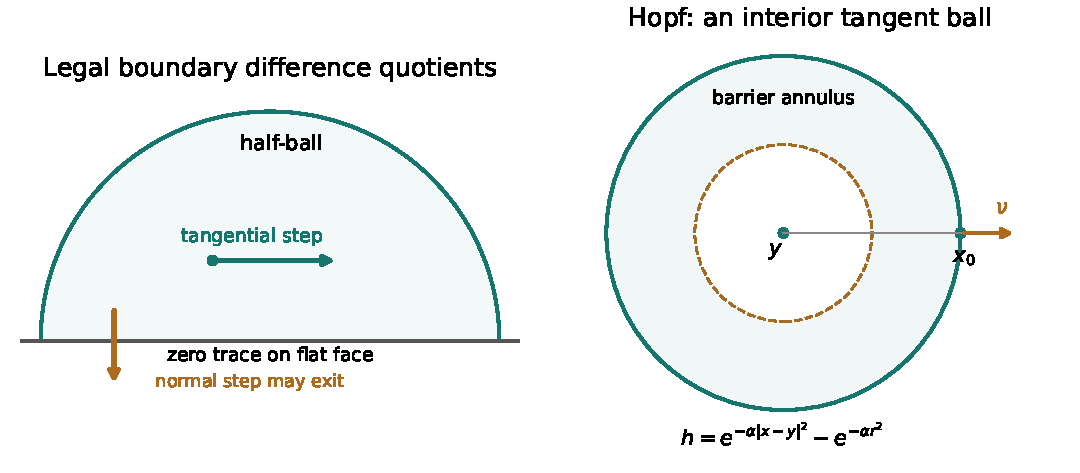
\includegraphics[width=\linewidth]{output/figures/ch06-boundary-tools.pdf}
\end{center}
{\small\textit{Two boundary mechanisms.} Tangential translations preserve
the flat zero-trace face; normal translations need not.
Hopf's exponential barrier is used only in the shaded annulus of an
interior tangent ball. Diagrams are schematic.}
\end{minipage}

\Needspace{35mm}
\subsection{Higher boundary regularity (Evans \S6.3.2, Theorems 5--6)}
\begin{theorem}\label{thm:6-higher-boundary}
If $\partial U$ is $C^{m+2}$, $A,b,c\in C^{m+1}(\overline U)$ and
$f\in H^m(U)$, then a weak zero-Dirichlet solution satisfies
\[
 u\in H^{m+2}(U),\qquad
 \|u\|_{H^{m+2}(U)}
 \leq C\bigl(\|f\|_{H^m(U)}+\|u\|_2\bigr).
\]
Smooth boundary, coefficients and data give $u\in C^\infty(\overline U)$.
\end{theorem}
\begin{expandedproof}
The case $m=0$ is Theorem~\ref{thm:6-boundary-h2}.
For the induction step assume $u\in H^{m+2}$ and $f\in H^{m+1}$,
with coefficients $C^{m+2}$ and boundary $C^{m+3}$.
In a flattened chart, differentiate $m+1$ times only tangentially.
The resulting derivative has zero trace on the flat face, because
tangential differentiation commutes with the trace at these orders.
Its localized equation has an $L^2$ right side: expand the commutators
exactly as in the interior proof. Cutoffs keep tests away from the
curved part of the chart. Applying boundary $H^2$ gives all derivatives
of total order $N=m+3$ having at most two normal differentiations.

Recover the others from \eqref{eq:6-normal-recovery}. To estimate an
order-$N$ derivative with $q\geq3$ normal indices, apply an order-$N-2$
derivative with $q-2$ normal indices to that identity.
The desired term is multiplied by $a^{nn}$; the other order-$N$ terms
have at most $q-1$ normal indices, and coefficient commutators contain
derivatives of $u$ of order at most $N-1$, already controlled.
Induct on $q$ and divide by $a^{nn}\geq\theta$.
These differentiated identities can be justified first by interior
regularity and then by the uniform estimates up to the flat face,
as in the $H^2$ case. Patching proves the global estimate.
Finally extend Sobolev functions across the smooth boundary and use
embedding at arbitrarily high orders to obtain $C^\infty(\overline U)$.
\end{expandedproof}
\Needspace{45mm}
\PDEAnnotation{边界光滑度不能省略}{内部正则性只看系数和右端，边界正则性还看区域形状。角点可能产生奇性；零边界条件本身并不能保证解在角点附近有平方可积的二阶导数。}
\paragraph{What the estimates actually say.}
The two-derivative gain is an a priori estimate for solutions, not an
existence theorem by itself. At an eigenvalue, the term $\|u\|_2$
cannot be removed: a nonzero eigenfunction solves a homogeneous
shifted equation. Nonzero boundary data require a sufficiently regular
lift before the zero-boundary theorem can be used.